\section{Nonmonotonic Rule Learning}\label{sec:nmrulelearn}
So far we have considered approaches that learn Horn rules. However,  Horn rules are not sufficiently expressive for representing incomplete human knowledge, and they are inadequate for capturing
exceptions. Thus, the rules extracted from the existing KGs can potentially %they %herefore, they 
predict erroneous facts as illustrated in Section~\ref{sec:intro}. 

In this section, we provide an overview of approaches for nonmonotonic rule learning extraction from incomplete data. 

As illustrated earlier in Section~\ref{subsec:ilp}, the traditional nonmonotonic inductive and abductive algorithms cannot be directly adopted for real-life KGs. So, recently \cite{gad2016} and its successor RUMIS~\cite{rumis} have been developed specifically to learn nonmonotonic rules from the large KGs, taking into account the OWA and the huge size of the KG. Both %\cite{gad2016} and RUMIS try to 
%learn exceptions from a learned rules set % in the KG 
%by revising % the set of Horn rules $R_H$ extracted from the KG
% into a nonmonotonic set $R_{MN}$ by
learn exceptions starting with a learned Horn rules set and revise it by  
adding at most one negated atom to each rule at a time. The revision is constructed such that the average quality of the Horn rule set is maximized, while the conflict among the predictions of the rules are minimized. To estimate this conflict ratio, the negative predictions are materialized. To this end, % herefore,
% they introduce 
the notion of an auxiliary rule for a given rule $r:H \leftarrow B, \naf E$ has been introduced as follows: % , concretely, for a rule 
%, the auxiliary version is 
$r^{aux}:\mi{not\_H} \leftarrow B, E$ where $\mi{not\_H}$ is a fresh predicate indicating that $H$ will not be derived by this rule. The number of grounded pairs $\tuple{H,\mi{not\_H}}$ in the answer set generated by the rule set, the auxiliary rules and the KG indicates the degree of conflict.

\begin{figure}[t]
\centering
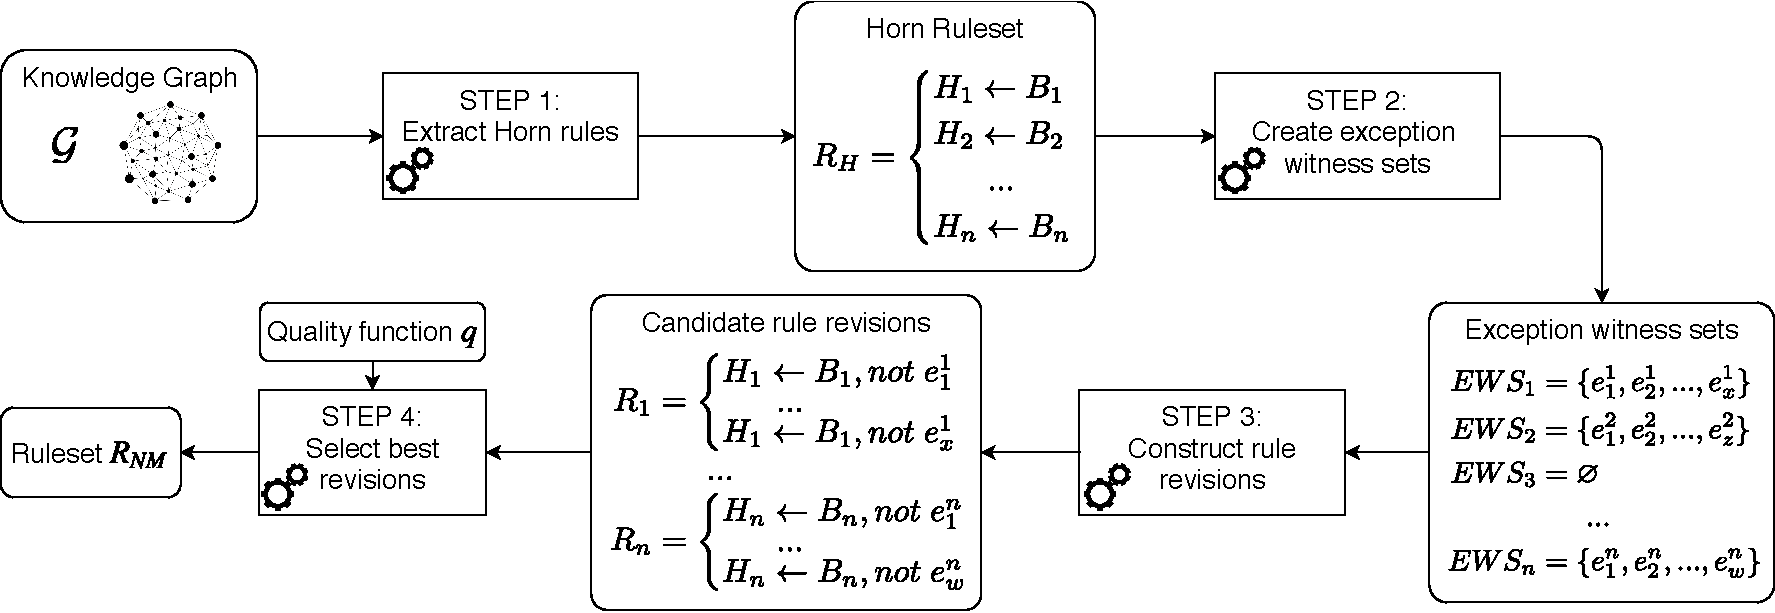
\includegraphics[width=1\textwidth]{figures/overview_new}
\caption{Rule revision process by~\cite{gad2016,rumis}.}
\label{fig:iswc_process}
\end{figure}

Figure~\ref{fig:iswc_process} shows the rule revision steps as described by~\cite{gad2016} (and similarly RUMIS). The first step is to extract the Horn rules from the KG. Since ~\cite{gad2016} only supports unary predicates, the KG is first projected from the binary relations into unary ones by introducing new predicates that combine the original predicate and the class of the object entity. For example, given facts $\mi{marriedTo(bob, alice)}$ and $\mi{researcher(alice)}$, the binary fact is projected into $\mi{marriedTo\_researcher(bob)}$. Not that substituting the object instance with one of its classes allows learning patterns. A traditional item set mining approach is utilized to obtain the Horn rules $R_H$ from the projected KG. RUMIS takes as input a rule set learned by other Horn rule mining system such as AMIE ~\cite{amie}.   


The second step is concerned with the construction of the exception witness set (EWS). To realize that, the normal and abnormal instances sets are defined for each rule $r$: the normal set is the substitutions of the variables $\mathcal{V}$ with the entities such that satisfy both the head and the body of the rule $r$, while the abnormal set contains the  substitutions for which the rule's  body is satisfied but not the head.
Formally, for each rule $r \in \cR_H$, let $\mathcal{V}$ be the set of variables of $r$, the normal and abnormal sets are respectively defined as follows:
\begin{itemize}
\item $NS(r, \cG) = \{\theta \mid head(r)\theta, body(r)\theta \subseteq \cG\}$
\item $ABS(r, \cG) = \{\theta \mid body(r)\theta \subseteq \cG , head(r)\theta \notin \cG\}$\\
where $\theta: \mathcal{V} \rightarrow \cC$.
\end{itemize}

\begin{example}
Consider the KG $\cG$ and $r_1$ from Figure~\ref{rdf} as before, the normal set for $r_1$ is $NS(r_1,\cG)=\{\theta_1, \theta_2 ,\theta_3\}$, where $\theta_1 = \{X/brad, Y/ann, Z/berlin\}$,\\  $\theta_2 = \{X/john, Y/kate, Z/chicago\}$ and $\theta_3 = \{X/sue, Y/li, Z/beijing\}$.\\ and the abnormal set, $ABS(r_1,\cG)=\{\theta_4,\theta_5, \theta_6\}$, \\such that $\theta_4=\{X/bob, Y/alice, Z/berlin\}$,  $\theta_5=\{X/clara, Y/dave, Z/chicago\}$, and $\theta_6=\{X/mat, Y/lucy, Z/amsterdam\}$.
\qed
\end{example}

EWS is then constructed from the relations distinguishing the abnormal set from the normal one. Formally, for each rule $r \in \cR_H$, given that $\mathcal{V}$ is a set of variables occurring in $r$ and $\mathcal{X} \subseteq \mathcal{V}$; then, the Exception Witness Set (EWS) of $r$ with respect to the KG and $X$ is  the maximal set of predicates $EWS(r,\cG,\mathcal{X}) = \{p_1,...,p_k\}$ such that:
\begin{itemize}
\item $\forall i \in \{1,..,k\} : \exists \theta \in ABS(r, \cG)\ s.t.\ p_i(\mathcal{X}\theta) \in \cG$, and 
\item $\forall \theta \in NS(r,\cG) :  p_1(\mathcal{X}\theta), ...,p_k(\mathcal{X}\theta) \notin \cG$
\end{itemize}

Following these constraints, $EWS(r,\cG,\mathcal{X})$ will contain all possible exceptions to be added to $r$ with respect to variables of $\mathcal{X}$ such that the exception is witnessed with the abnormal substitutions but not the normal ones.


\begin{example}
Recalling $\cG$ and $r_1$, the exceptions witness sets for both variable $X$ and $Y$ are $EWS(r_1,\cG,\{X\}) = \{artist\}$ and $EWS(r_1,\cG,\{Y\}) = \{researcher\}$, respectively.
\qed
\end{example}
For each rule $r \in \cR_H$, the EWSs are collected in one set $EWS(r,\cG)$ containing all of its exception candidates. 
%\[EWS(r,\cG)=\bigcup_{\forall\mathcal{X}\subseteq \mathcal{V}}EWS(r,\cG,\mathcal{X})\] 

For the third and fourth steps in Figure~\ref{fig:iswc_process}, instead of creating all possible revisions then searching for the optimum revision $R_{NM}$, a local approach is proposed to pick the best revision for each rule $r \in R_H$. Several exception scoring functions have been proposed to select the best revision locally:
\begin{itemize}
\item \textbf{Naive}: It is the direct way of choosing the revision using only some standard measure such as confidence or conviction.
\item \textbf{PM}: Intuitively, the idea behind the \textit{partial materialization} is to rank candidate revisions based on its extension with predictions produced by other rules in $R_H$ (\ie partially materialized); hence, ensuring a cross-talk between the rules.
\item \textbf{OPM}: The \textit{ordered partial materialization} is similar to \textbf{PM}, but only materialize the rules of $\cR_{H}$ with higher quality than the current rule.
\item \textbf{OWPM}: The \textit{ordered weighted partial materialization} distinguishes between the original facts in the KG and the partial materialization facts by assigning a weight for the materialized facts inherited from the rules used to generate them. 
\end{itemize}


 %\gad{stopped here! details to be added}
 

